\chapter{The Epsilon Validation Language (EVL)}
\label{sec:EVL}

The aim of EVL is to contribute model validation capabilities to Epsilon. More specifically, EVL can be used to specify and evaluate constraints on models of arbitrary metamodels and modelling technologies. This section provides a discussion on the motivation for implementing EVL, its abstract and concrete syntax as well as its execution semantics. It also provides two examples using the language to verify inter-model and intra-model consistency.

\section{Motivation}
\label{sec:OCL.Limitations}

Although many approaches have been proposed to enable automated model validation, the Object Constraint Language (OCL) \cite{OCL} is the de facto standard for capturing constraints in modelling languages specified using object-oriented metamodelling technologies. While its powerful syntax enables users to specify meaningful and concise constraints, its purely declarative and side-effect free nature introduces a number of limitations in the context of a contemporary model management environment. In this section, the shortcomings of OCL that have motivated the design of EVL are discussed in detail.

In OCL, structural constraints are captured in the form of \textit{invariants}. Each invariant is defined in the context of a meta-class of the metamodel and specifies a name and a body. The body is an OCL expression that must evaluate to a \emph{Boolean} result, indicating whether an instance of the meta-class satisfies the invariant or not. Execution-wise, the body of each invariant is evaluated for each instance of the meta-class and the results are stored in a set of $<$Element, Invariant, Boolean$>$ triplets. Each triplet captures the \emph{Boolean} result of the evaluation of an \emph{Invariant} on a qualified \emph{Element}. An exemplar OCL invariant for UML 1.4, requiring that abstract operations only belong to abstract classes, is shown in Listing \ref{lst:AbstractOperations}.

\begin{lstlisting}[float=tbp, caption=OCL constraint on UML operations, label=lst:AbstractOperations, language=OCL]
context Operation
  inv AbstractOperationInAbstractClassOnly :
    self.isAbstract implies self.owner.isAbstract
\end{lstlisting}

While in its current version OCL enables users to capture particularly complex invariants, it also demonstrates a number of shortcomings, as follows.

\subsection{Limited user feedback}
\label{sec:Issue1}
OCL does not support specifying meaningful messages that can be reported to the user in case an invariant is not satisfied for certain elements. Therefore, feedback to the user is limited to the name of the invariant and the instance(s) for which it failed. Weak support for proper feedback messages implies that the end users must be familiar with OCL so that they can comprehend the meaning of the failed invariant and locate the exact reason for the failure. This is a significant shortcoming as in practice only a very small number of end users are familiar with OCL.

\subsection{No support for warnings/critiques}
\label{sec:Issue2}
Contemporary software development environments typically produce two types of feedback when checking artefacts for consistency and correctness: errors and warnings. Errors indicate critical deficiencies that contradict basic principles and invalidate the developed artefacts. By contrast, warnings (or critiques) indicate non-critical issues that should nevertheless be addressed by the user. To enable users to address warnings in a priority-based manner, they are typically categorized into three levels of importance: High, Medium and Low (although other classifications are also possible).

Nevertheless, in OCL there is no such distinction between errors and warnings and consequently all reported issues are considered to be errors. This adds an additional burden to identifying and prioritizing issues of major importance, particularly within an extensive set of unsatisfied invariants in complex models.

\subsection{No support for dependent constraints}
\label{sec:Issue3}
Each OCL invariant is a self-contained unit that does not depend on other invariants. There are cases where this design decision is particularly restrictive. For instance consider the invariants \emph{I1} and \emph{I2} displayed in Listing \ref{lst:RelatedConstraints}. Both I1 and I2 are applicable on UML classes with \emph{I1} requiring that: \textit{the name of a class must not be empty} and \emph{I2} requiring that: \textit{the name of a class must start with a capital letter}. In the case of those two invariants, if \emph{I1} is not satisfied for a particular UML class, evaluating \emph{I2} on that class would be meaningless. In fact it would be worse than meaningless since it would consume time to evaluate and would also produce an extraneous error message to the user. In practice, to avoid the extraneous message, \emph{I2} needs to replicate the body of \emph{I1} using an \textit{if} expression (lines 2 and 5).

\begin{lstlisting}[float=tbp, caption=Conceptually related OCL constraints, label=lst:RelatedConstraints, language=OCL]
context Class
	inv I1 : self.name.size() > 0
    	
  inv I2 : 
		if self.name.size > 0 then
			self.name.substring(0,1) =
			self.name.substring(0,1).toUpper()
		else
			true
		endif
\end{lstlisting}

\subsection{Limited flexibility in context definition}
\label{sec:Issue4}
As already discussed, in OCL invariants are defined in the context of meta-classes. While this achieves a reasonable partitioning of the model element space, there are cases where more fine-grained partitioning is required. For instance, consider the following scenario. Let $IA_{1..N}$, $IB_{1..M}$ be invariants applying to classes that are stereotyped as \verb|<<A>>| and \verb|<<B>>| respectively. Since OCL only supports partitioning the model element space using meta-classes, all $IA_{1..N}$, $IB_{1..M}$ must appear under the same context (i.e. \textit{Class}). Moreover, each invariant must explicitly define that it addresses the one or the other conceptual sub-partition. Therefore, each of $IA_{1..N}$ must limit its scope initially (using the $self.isA$ expression) and then express the real body. In our example the simplest way to achieve this would be by combining a scope-limiting expression with the real invariant body using the \textit{implies} clause as demonstrated in Listing \ref{lst:OCLDuplication}.

\begin{lstlisting}[float=tbp, caption=Demonstration of OCL constraints with duplication, label=lst:OCLDuplication, language=OCL2]
context Class
	inv I1 : self.isA implies <real-invariant-body>
	inv I2 : self.isA implies <real-invariant-body>
	...
	inv IN : self.isA implies <real-invariant-body>
	
	def isA :
		let isA : Boolean = 
		self.stereotype->exists(s|s.name = 'A')
\end{lstlisting}

Furthermore, if the \emph{real} body of the invariant needs to assume that self is stereotyped with \verb|<<A>>|, this technique is not applicable because OCL does not support lazy evaluation of Boolean clauses \cite{OCL} and therefore although the first part of the expression (\verb|self.isA|) may fail for some instances, the second part will still be evaluated thus producing runtime errors. In this case, an \textit{if} expression must be used, further complicating the specified invariants.

\subsection{No support for repairing inconsistencies} 
\label{sec:Issue5}
While OCL can be used for detecting inconsistencies, it provides no means for repairing them. The reason is that OCL has been designed as a side-effect free language and therefore lacks constructs for modifying models. Nevertheless, there are many cases where inconsistencies are trivial to resolve and users can benefit from semi-automatic repairing facilities. 

This need has been long recognized in the related field of code development tools (e.g. Eclipse, Microsoft Visual Studio, NetBeans). In such tools, errors are not only identified but also context-aware actions are proposed to the user for automatically repairing them. This feature significantly increases the usability of such tools and consequently enhances users' productivity.\\

\subsection{No support for inter-model constraints}
\label{sec:Issue6}
OCL expressions (and therefore OCL constraints) can only be evaluated in the context of a single model at a time. Consequently, OCL cannot be used to express constraints that span across different models. In the context of a large-scale model driven engineering process that involves many different models (that potentially conform to different modelling languages) this limitation is particularly severe.\\

\noindent Following this discussion on the shortcomings of OCL for capturing structural constraints in modelling languages, the following sections present the abstract and concrete syntax of EVL as well as their execution semantics, and explain how they address the aforementioned limitations.

\section{Abstract Syntax}

In EVL, validation specifications are organized in modules (\emph{EvlModule}). As illustrated in Figure \ref{fig:EvlAbstractSyntax}, \emph{EvlModule} extends \emph{EolLibraryModule} which means that it can contain user-defined operations and import other EOL library modules and EVL modules. Apart from operations, an EVL module also contains a set of invariants grouped by the context they apply to, and a number of \emph{pre} and \emph{post} blocks.

\begin{landscape}
\begin{figure}
	\centering
	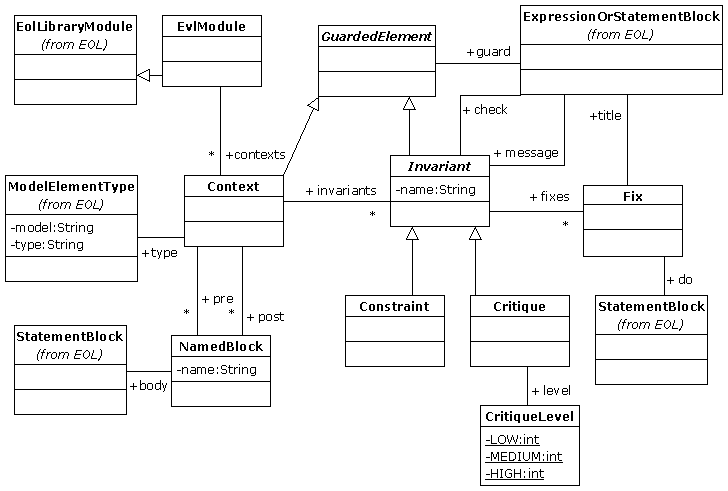
\includegraphics{images/EvlAbstractSyntax.png}
	\caption{Abstract Syntax of EVL}
	\label{fig:EvlAbstractSyntax}
\end{figure}
\end{landscape}

\paragraph{Context} A context specifies the kind of instances on which the contained invariants will be evaluated. Each context can optionally define a guard which limits its applicability to a narrower subset of instances of its specified type. Thus, if the guard fails for a specific instance of the type, none of its contained invariants are evaluated.

\paragraph{Invariant} As with OCL, each EVL invariant defines a \emph{name} and a body (\emph{check}). However, it can optionally also define a \emph{guard} (defined in its abstract \emph{GuardedElement} supertype) which further limits its applicability to a subset of the instances of the type defined by the embracing \emph{context}. To achieve the requirement for detailed user feedback (Section \ref{sec:Issue1}), each invariant can optionally define a \emph{message} as an \emph{ExpressionOrStatementBlock} that should return a String providing a description of the reason(s) for which the constraint has failed on a particular element. To support semi-automatically fixing of elements on which invariants have failed (Section \ref{sec:Issue5}), an invariant can optionally define a number of \emph{fixes}. Finally, as displayed in Figure \ref{fig:EvlAbstractSyntax}, \emph{Invariant} is an abstract class that is used as a super-class for the specific types \emph{Constraint} and \emph{Critique}. This is to address the issue of separation of errors and warnings/critiques (Section \ref{sec:Issue2}).

\paragraph{Guard} Guards are used to limit the applicability of invariants (Section \ref{sec:Issue4}). This can be achieved at two levels. At the \emph{Context} level it limits the applicability of all invariants of the context and at the \emph{Invariant} level it limits the applicability of a specific invariant.

\paragraph{Fix}
A fix defines a title using an \emph{ExpressionOrStatementBlock} instead of a static String to allow users to specify context-aware titles (e.g. \emph{Rename class customer to Customer} instead of a generic \emph{Convert first letter to upper-case}). Moreover, the \emph{do} part is a statement block where the fixing functionality can be defined using EOL. The developer is responsible for ensuring that the actions contained in the \emph{fix} actually repair the identified inconsistency.

\paragraph{Constraint}
\emph{Constraints} in EVL are used to capture critical errors that invalidate the model. As discussed above, \emph{Constraint} is a sub-class of \emph{Invariant} and therefore inherits all its features.

\paragraph{Critique}
Unlike \emph{Constraints}, \emph{Critiques} are used to capture non-critical situations that do not invalidate the model, but should nevertheless be addressed by the user to enhance the quality of the model. This separation addresses the issue raised in Section \ref{sec:Issue2}. Moreover, to enable users to define different levels of importance in critiques, the \emph{CritiqueLevel} enumeration supports a 3-level classification. Fixed-level classification has been preferred in EVL over infinite level classification (e.g. using Integer levels) since it is more common in development tools and easier to visualize.

\paragraph{Pre and Post}
An EVL module can define a number of named \emph{pre} and a \emph{post} blocks that contain EOL statements which are executed before and after evaluating the invariants respectively.

\section{Concrete Syntax}

Listings \ref{lst:ContextConcreteSyntax}, \ref{lst:InvariantConcreteSyntax} and \ref{lst:FixConcreteSyntax} demonstrate the concrete sytnax of the \emph{context}, \emph{invariant} and \emph{fix} abstract syntax constructs discussed above.

\begin{lstlisting}[float=tbp, caption=Concrete Syntax of an EVL context, label=lst:ContextConcreteSyntax, language=EVL, escapechar=!]

context !\textit{name}! !\textbf{\{}!

	(guard (!\textbf{:}\textit{expression}!)|(!\textbf{\{}\textit{statementBlock}\textbf{\}}!))?
	
	(!\textit{invariant}!)*
	
!\textbf{\}}!
\end{lstlisting}

\begin{lstlisting}[float=tbp, caption=Concrete Syntax of an EVL invariant, label=lst:InvariantConcreteSyntax, language=EVL, escapechar=!]

(@lazy)?
(constraint|critique) !\textit{name}! !\textbf{\{}!
	
	(guard (!\textbf{:}\textit{expression}!)|(!\textbf{\{}\textit{statementBlock}\textbf{\}}!))?
	
	(check (!\textbf{:}\textit{expression}!)|(!\textbf{\{}\textit{statementBlock}\textbf{\}}!))?
	
	(message (!\textbf{:}\textit{expression}!)|(!\textbf{\{}\textit{statementBlock}\textbf{\}}!))?
	
	(!\textit{fix}!)*
	
!\textbf{\}}
\end{lstlisting}

\begin{lstlisting}[float=tbp, caption=Concrete Syntax of an EVL fix, label=lst:FixConcreteSyntax, language=EVL, escapechar=!]
fix !\textbf{\{}!
	
	(guard (!\textbf{:}\textit{expression}!)|(!\textbf{\{}\textit{statementBlock}\textbf{\}}!))?
	
	(title (!\textbf{:}\textit{expression}!)|(!\textbf{\{}\textit{statementBlock}\textbf{\}}!))?
	
	do !\textbf{\{}!
		!\textit{statementBlock}!
	!\textbf{\}}!
	
!\textbf{\}}!
\end{lstlisting}

\emph{Pre} and \emph{post} blocks have a simple syntax that, as presented in Listing \ref{lst:EvlPrePostConcreteSyntax}, consists of the identifier (\emph{pre} or \emph{post}), an optional name and the set of statements to be executed enclosed in curly braces.

\begin{lstlisting}[float=tbp, caption=Concrete Syntax of Pre and Post blocks, label=lst:EvlPrePostConcreteSyntax, language=EVL]
(pre|post) <name> {
	statement+
}
\end{lstlisting}

%\subsection{Concepts reused from EOL}

%As EVL has been built atop EOL, it reuses the following constructs from the base-language:

%\paragraph{ExpressionOrStatementBlock} There are cases where users needs to calculate a value (e.g. in the \emph{message} of an \emph{invariant}, in the \emph{guard} of a \emph{context} etc). When the value can be calculated declaratively, this is preferred. However, for cases in which calculating the value requires complex computations, users can use an EOL statement block and use a \emph{ReturnStatement} to return the calculated value to the caller.

%\paragraph{StatementBlock} A statement block is a sequence of EOL statements that can optionally include one or more \emph{ReturnStatements} to return a calculated value to its caller.

\section{Execution Semantics}
\label{sec:Design.EVL.ExecutionSemantics}

Having discussed the abstract and concrete syntaxes of EVL, this section provides an informal discussion of the execution semantics of the language. The execution of an EVL module is separated into four phases:

%The additional concepts EVL provides also affect its execution semantics. Currently, an EVL module can only be executed in batch-mode (all invariants against all instances). In the future we plan to investigate how the additional structures that EVL provides affect approaches to incremental consistency checking such as those presented in \cite{Cabot06,Egyed06}. In this section we outline the execution semantics of the language in batch-mode.

\paragraph{Phase 1} Before any invariant is evaluated, the \emph{pre} sections of the module are executed in the order in which they have been specified.

\paragraph {Phase 2} For each \emph{context}, the instances of the meta-class it defines are collected. For each instance, the \emph{guard} of the \emph{context} is evaluated. If the \emph{guard} is satisfied, then for each non-lazy invariant contained in the context the invariant's \emph{guard} is also evaluated. If the \emph{guard} of the invariant is satisfied, the \emph{body} of the invariant is evaluated. In case the \emph{body} evaluates to \emph{false}, the \emph{message} part of the rule is evaluated and the produced message is added along with the instance, the invariant and the available \emph{fixes} to the \emph{ValidationTrace}. 

The execution order of an EVL module follows a top-down depth-first scheme that respects the order in which the \emph{contexts} and \emph{invariants} appear in the module. However, the execution order can change in case one of the \emph{satisfies}, \emph{satisfiesOne}, \emph{satisfiesAll} built-in operations, discussed in detail in the sequel, are called.

\paragraph{Phase 3} In this phase, the validation trace is examined for unsatisfied constraints and the user is presented with the message each one has produced. The user can then select one or more of the available \emph{fixes} to be executed. Execution of \emph{fixes} is performed in a transactional manner using the respective facilities provided by the model connectivity framework, as discussed in Section \ref{sec:EMC.ModelTransactionSupport}. This is to prevent runtime errors raised during the execution of a \emph{fix} from compromising the validated model by leaving it in an inconsistent state.

\paragraph{Phase 4} When the user has performed all the necessary \emph{fixes} or chooses to end Phase 3 explicitly, the \emph{post} section of the module is executed. There, the user can perform tasks such as serializing the validation trace or producing a summary of the validation process results.

\subsection{Capturing Dependencies Between Invariants}

As discussed in Section \ref{sec:Issue3}, it is often the case that invariants conceptually depend on each other. To allow users capture such dependencies, EVL provides the \emph{satisfies(invariant : String) : Boolean}, \emph{satisfiesAll(invariants : Sequence(String)) : Boolean} and \emph{satisfiesOne(invariants : Sequence(String)) : Boolean} built-in operations. Using these operations, an invariant can specify in its \emph{guard} other invariants which need to be satisfied for it to be meaningful to evaluate.

When one of these operations is invoked, if the required \emph{invariants} (either lazy or non-lazy) have been evaluated for the instances on which the operation is invoked, the engine will return their cached results; otherwise it will evaluate them and return their results.

\section{Intra-Model Consistency Checking Example}
\label{sec:EvlIntraModelExample}
This section presents a case study comparing EVL and OCL in the context of a common scenario. The purpose of the case study is to present readers with the concrete syntax of the language and demonstrate the benefits delivered by the additional constructs it facilitates.

\subsection{Scenario: The Singleton Pattern}

The \emph{singleton} pattern is a widely used object oriented pattern. A \emph{singleton} is a class for which \emph{exactly one instance is allowed} \cite{Larman}. In UML, a singleton is typically represented as a class which is stereotyped with a \verb|<<singleton>>| stereotype and which also defines a static operation named \emph{getInstance()} that returns the unique instance. 

To ensure that all singletons have been modelled correctly in a UML model one needs to evaluate the following invariants on all classes that are stereotyped with the \verb|<<singleton>>| stereotype:

\begin{itemize}
	\item DefinesGetInstance : Each stereotyped class must define a getInstance() method
	\item GetInstanceIsStatic : The getInstance() method must be static
	\item GetInstanceReturnsSame : The return type of the getInstance() method must be the class itself 
\end{itemize}

Obviously, invariants \emph{GetInstanceIsStatic} and \emph{GetInstanceReturnsSame} depend on \emph{DefinesGetInstance} because if the singleton does not define a \emph{getInstance()} operation, checking for the operation's scope and return type is meaningless. Moreover, in case an invariant fails, there are corrective actions (fixes) that users may want to perform semi-automatically: e.g. for \emph{DefinesGetInstance}, such an action would be to add the missing \emph{getInstance()} operation, for \emph{GetInstanceIsStatic} to change it to static and for \emph{GetInstanceRetunrsSame} to set the return type to the class itself. In the following sections OCL and EVL are used to express the three constraints and then the two solutions are compared.

\subsection{Using OCL to Express the Invariants}

Listing \ref{lst:CaseStudyOcl} shows the aforementioned invariants implemented in OCL.

\begin{lstlisting}[basicstyle=\ttfamily\footnotesize, flexiblecolumns=true, numbers=none, nolol=true, caption=OCL Module for Validating Singletons, label=lst:CaseStudyOcl, numbers=left, language=OCL2, tabsize=2]
package Foundation::Core
    
		context Class 

		def isSingleton :
			let isSingleton : Boolean =
			self.stereotype->exists(s|s.name = 'singleton')
        
		def getInstanceOperation  : 
			let getInstanceOperation : Operation =
			self.feature->select(f|f.oclIsTypeOf(Operation) 
			and f.name = 'getInstance')->first().oclAsType(Operation)

		inv DefinesGetInstanceOperation : 
			if isSingleton 
				then getInstanceOperation.isDefined
				else true
			endif
    	
		inv GetInstanceOperationIsStatic :
			if isSingleton then
				if getInstanceOperation.isDefined 
					then getInstanceOperation.ownerScope = #classifier 
					else false
				endif
			else 
				true
			endif
    	
		inv GetOperationReturnsSame :
			if isSingleton then
				if getInstanceOperation.isDefined then
					if getInstanceOperation.returnParameter.isDefined
						then getInstanceOperation.returnParameter.type = self 
						else false
					endif
				else
					false
				endif
			else 
				true
			endif
    	
    context Operation
        
		def returnParameter :
			let returnParameter : Parameter =
			self.parameter->select(p|p.kind = #return)->first()

endpackage

\end{lstlisting}

By examining the OCL solution it can be observed that all invariants first check that the class is a singleton (lines 15, 21 and 31) by using the \emph{isSingleton} derived property defined in line 5. If the isSingleton returns \emph{false}, the invariants return \emph{true} since returning false would cause them to fail for all non-singleton classes. This reveals an additional shortcoming of OCL: if a constraint returns \emph{true} it may mean two different things: either that the instance satisfies the constraint or that the constraint is not applicable to the instance at all. In our view, this overloading reduces understandability.

By further studying the solution of Listing \ref{lst:CaseStudyOcl} it can be noticed that dependency between constraints is captured artificially using nested \emph{if} expressions. For instance, both \emph{GetInstanceIsStatic} and \emph{GetInstanceRetunrsSame} contain an \emph{if} expression in lines 22 and 32 respectively, requiring that they recalculate the value of the \emph{getInstanceOperation} defined in line 9, where they actually recalculate the result of the \emph{DefinesGetInstanceOperation} invariant. As discussed in Section \ref{sec:Issue3}, this happens because OCL lacks constructs for capturing dependencies in a structured manner.

\subsection{Using EVL to Express the Invariants}

Listing \ref{lst:CaseStudy} provides a solution for this problem expressed in EVL.

\begin{lstlisting}[basicstyle=\ttfamily\footnotesize, flexiblecolumns=true, numbers=none, nolol=true, caption=EVL Module for Validating Singletons, label=lst:CaseStudy, numbers=left, language=EVL, tabsize=2]
context Singleton typeOf Class {
	
	guard : self.stereotype->exists(s|s.name = 'singleton')
	
	constraint DefinesGetInstance {
		check : self.getGetInstanceOperation()->isDefined()
		message : 'Singleton ' + self.name + 
			' must define a getInstance() operation'
		fix {
			title : 'Add a getInstance() operation to ' + self.name
			do {
				-- Create the getInstance operation
				var op : new Operation;
				op.name := 'getInstance';
				op.owner := self;
				op.ownerScope := ScopeKind#sk_classifier;
				
				-- Create the return parameter
				var returnParameter : new Parameter;
				returnParameter.type := self;
				op.parameter := Sequence{returnParameter};
				returnParameter.kind := ParameterDirectionKind#pdk_return;
			}
		}
	}
	
	constraint GetInstanceIsStatic {
		guard : self.satisfies('DefinesGetInstance')
		check : self.getGetInstanceOperation().ownerScope = 
		        ScopeKind#sk_classifier
		message : ' The getInstance() operation of singleton ' 
		          + self.name + ' must be static'
	
		fix {
			title : 'Change to static'
			do {
				self.getGetInstanceOperation.ownerScope 
				  := ScopeKind#sk_classifier;
			}
		}
	}
	
	constraint GetInstanceReturnsSame {
	
		guard : self.satisfies('DefinesGetInstance')
		check {
			var returnParameter : Parameter;
			returnParameter := self.getReturnParameter();
			return (returnParameter->isDefined() 
			        and returnParameter.type = self);
		}
		message : ' The getInstance() operation of singleton ' 
		          + self.name + ' must return ' + self.name
			
		fix {
			title : 'Change return type to ' + self.name
			do {
				var returnParameter : Parameter;
				returnParameter := self.getReturnParameter();
				
				-- If the operation does not have a return parameter
				-- create one
				if (not returnParameter.isDefined()){
					returnParameter := Parameter.newInstance();
					returnParameter.kind := ParameterDirectionKind#pdk_return;
					returnParameter.behavioralFeature := 
						self.getInstanceOperation();
				}
				-- Set the correct return type
				returnParameter.type := self;
			}
		}
	}
}

operation Class getGetInstanceOperation() : Operation {
	return self.feature->
		select(o:Operation|o.name = 'getInstance').first();
}

operation Operation getReturnParameter() : Parameter {
	return self.parameter->
		select(p:Parameter|p.kind = 
			ParameterDirectionKind#pdk_return).first();
}
\end{lstlisting}

The \emph{Singleton} context defines that the invariants it contains will be evaluated on instances of the UML \emph{Class} type. Moreover, its guard defines that they will be evaluated only on classes that are stereotyped with the \emph{singleton} stereotype. Therefore, unlike the OCL solution of Listing \ref{lst:CaseStudyOcl}, invariants contained in this context do not need to check individually that the instances on which they are evaluated are singletons.

Constraint \emph{DefinesGetInstance} defines no guard which means that it will be evaluated for all the instances of the context. In its \emph{check} part, the constraint examines if the class defines an operation named \emph{getInstance()} by invoking the \emph{getGetInstanceOperation()} operation. If this fails, it proposes a fix that adds the missing operation to the class.

Constraint \emph{GetInstanceIsStatic} defines a guard which states that for the constraint to be evaluated on an instance, the instance must first satisfy the \emph{DefinesGetInstance} constraint. If it doesn't, it is not evaluated at all. In its \emph{check} part it examines that the \emph{getInstance()} operation is static. Note that here the constraint needs not check that the \emph{getInstance()} operation is defined again since this is assumed by the \emph{DefinesGetInstance} constraint on which it depends. If the constraint fails for an instance, the fix part can be invoked to change the scope of the \emph{getInstance()} operation to static.

Constraint \emph{GetInstanceReturnsSame} checks that the return type of the \emph{getInstance()} operation is the singleton itself. Similarly to the \emph{GetInstanceIsStatic} constraint, it defines that to be evaluated the \emph{DefinesGetInstance} constraint must be satisfied. If it fails for a particular instance, the fix part can be invoked. In the fix part, if the operation defines a return parameter of incorrect type, its type is changed and if it does not define a return parameter at all, the parameter is created and added to the parameters of the operation.

By observing the two solutions the OCL solution resembles the concept of defensive programming, where conditions are embedded in supplier code, while the EVL one is closer to the design by contract \cite{Meyer97} approach where conditions are explicitly checked in guards.

This case study has demonstrated that the additional constructs provided by EVL can reduce repetition significantly and thus enable specification of more concise constraints. Moreover, in case a constraint is not satisfied for a particular instance, the user is provided with a meaningful context-aware message and with automated facilities (fixes) for repairing the inconsistency.

\section{Inter-Model Consistency Checking Example}
\label{sec:EvlInterModelExample}

In the previous example, EVL was used to check the internal consistency of a single UML model. By contrast, this example demonstrates using EVL to detect and repair occurrences of incompleteness and contradiction between two different models. In this example the simplified \emph{ProcessLang} metamodel, which captures information about hierarchical processes, is used. To add performance information in a separate aspect \emph{ProcessPerformanceLang} metamodel is also defined. The metamodels are displayed in Figures \ref{fig:Process} and \ref{fig:ProcessPerformance} respectively.

There are two constraints that need to be defined and evaluated in this example: that each \emph{Process} in a process model (\emph{PM}) has a corresponding \emph{ProcessPerformance} in the process performance model (\emph{PPM}), and that the \emph{maxAcceptableTime} of a process does not exceed the sum of the \emph{maxAcceptableTimes} of its children. This is achieves with the \emph{PerformanceIsDefined} and the \emph{PerformanceIsValid} EVL constraints displayed in Listing \ref{lst:InterModelCaseStudy}.

\begin{figure}
	\centering
		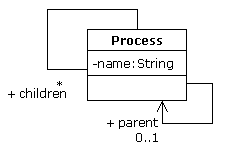
\includegraphics{images/Process.png}
	\caption{The ProcessLang Metamodel}
	\label{fig:Process}
\end{figure}

\begin{figure}
	\centering
		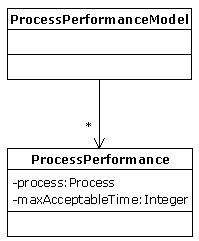
\includegraphics{images/ProcessPerformance.png}
	\caption{The ProcessPerformanceLang Metamodel}
	\label{fig:ProcessPerformance}
\end{figure}

\begin{lstlisting}[float=tbp, caption=Exemplar EVL module containing a cross-model constraint, label=lst:InterModelCaseStudy, language=EVL]
context PM!Process {
	
	constraint PerformanceIsDefined { /*@\label{CaseStudy:PerformanceIsDefined}@*/
		
		check { /*@\label{CaseStudy:PerformanceIsDefined:Check}@*/
			var processPerformances = 
				PPM!ProcessPerformance.
				allInstances.select(pt|pt.process = self);
			
			return processPerformances.size() = 1;
		}
		
		message { /*@\label{CaseStudy:PerformanceIsDefined:Message}@*/
			var prefix : String;
			if (processPerformances.size() = 1) {
				prefix = "More than one performance info"; 
			}
			else {
				prefix = "No performance info";
			}
			return prefix + " found for process " 
				+ self.name;
		}
		
		fix { /*@\label{CaseStudy:PerformanceIsDefined:Fix}@*/
			title : "Set the performance of " + self.name
			
			do {
				for (p in processPerformances.clone()) {
					delete p;
				}
				var maxAcceptableTime : Integer;
				maxAcceptableTime = UserInput. /*@\label{CaseStudy:PerformanceIsDefined:Fix:Prompt}@*/
					promptInteger("maxAcceptableTime", 0); 
				var p : 
					new PPM!ProcessPerformance;
				p.maxAcceptableTime = maxAcceptableTime;
				p.process = self;
			}
		}
	}
	
	constraint PerformanceIsValid { /*@\label{CaseStudy:PerformanceIsValid}@*/
		
		guard : self.satisfies("PerformanceIsDefined") /*@\label{CaseStudy:PerformanceIsValid:Guard}@*/
			and self.children.forAll
				(c|c.satisfies("PerformanceIsDefined"))
		
		check { /*@\label{CaseStudy:PerformanceIsValid:Check}@*/
			var sum : Integer;
			sum = self.children. /*@\label{CaseStudy:PerformanceIsValid:Sum}@*/
				collect(c|c.getMaxAcceptableTime()) 
				.sum().asInteger(); 
			return self.getMaxAcceptableTime() >= sum;
		}
		
		message : "Process " + self.name + /*@\label{CaseStudy:PerformanceIsValid:Message}@*/
			" has a smaller maxAcceptableTime " 
			+ "than the sum of its children"
		
		fix { /*@\label{CaseStudy:PerformanceIsValid:Fix}@*/
			title : "Increase maxAcceptableTime to " + sum
			do {
				self.setMaxAcceptableTime(sum);
			}
		}
		
	}
	
}

operation PM!Process getMaxAcceptableTime() /*@\label{CaseStudy:getMaxAcceptableTime}@*/
	: Integer { 
	return PPM!ProcessPerformance.
		allInstances.selectOne(pt|pt.process=self)
			.maxAcceptableTime;
}

operation PM!Process setMaxAcceptableTime /*@\label{CaseStudy:setMaxAcceptableTime}@*/
	(time : Integer) { 
	PPM!ProcessPerformance.allInstances.
		selectOne(pt|pt.process=self).maxAcceptableTime =
		time;
}
\end{lstlisting}

In line \ref{CaseStudy:PerformanceIsDefined:Check}, the check part of the \emph{PerformanceIsDefined} constraint calculates the instances of \emph{ProcessPerformance} in the \emph{ProcessPerformanceModel} that have their \emph{process} reference set to the currently examined \emph{Process} (accessible via the \emph{self} built-in variable) and stores it in the \emph{processPerformances} variable. If exactly one \emph{ProcessPerformance} is defined for the \emph{Process}, the constraint is satisfied. Otherwise, the \emph{message} part of the constraint, in line \ref{CaseStudy:PerformanceIsDefined:Message}, is evaluated and an appropriate error message is displayed to the user. 

Note that the \emph{processPerformances} variable defined in the \emph{check} part is also used from within the \emph{message} part of the constraint. As discussed in \cite{EVL}, EVL provides this feature to reduce the need for duplicate calculations as our experience has shown that the message for a failed constraint often needs to utilize side-information collected in the \emph{check} part.

To repair the inconsistency, the user can invoke the \emph{fix} defined in line \ref{CaseStudy:PerformanceIsDefined:Fix} that will delete any existing \emph{ProcessPerformance} instances and create a new one with a user-defined \emph{maxAcceptableTime} obtained using the \emph{UserInput.promptInteger()} statement of line \ref{CaseStudy:PerformanceIsDefined:Fix:Prompt}.

Unlike the \emph{PerformanceIsDefined} constraint, the \emph{PerformanceIsValid} constraint, line \ref{CaseStudy:PerformanceIsValid}, defines a \emph{guard} part (line \ref{CaseStudy:PerformanceIsValid:Guard}). As discussed in \cite{EVL}, the guard part of a constraint is used to further limit the applicability of the constraint beyond the simple type check performed in the containing \emph{context}. In this rule, the validity of the \emph{maxAcceptableTime} of a \emph{Process} needs to be checked only if one has been defined in the \emph{ProcessPerformanceModel}. Therefore, the guard part of the constraint specifies that this constraint is only applicable to \emph{Processes} where, both they and they children, satisfy the \emph{PerformanceIsDefined} constraint.

The check part of the constraint retrieves the \emph{maxAcceptableTime} of the process and that of its children and compares them. As the \emph{Process} itself does not define performance information, retrieval of the value of the \emph{maxAcceptableTime} of the respective \emph{ProcessPerformance} object is implemented using the user-defined \emph{getMaxAcceptableTime()} operation that is defined in line \ref{CaseStudy:getMaxAcceptableTime}. In case the constraint is not satisfied, the user can invoke the \emph{fix} defined in line \ref{CaseStudy:PerformanceIsValid:Fix} to repair the inconsistency by setting the \emph{maxAcceptableTime} of the process to the \emph{sum} calculated in line \ref{CaseStudy:PerformanceIsValid:Sum}. As discussed earlier, the fix parts of EVL invariants do not in any way guarantee that they do fix the problem they target or that in their effort to fix one problem they do not create another problem; this is left to the user. For instance, in this particular example, changing the \emph{maxAcceptableTime} of a process through a \emph{fix} block may render its parent process invalid.

\begin{figure*}
	\centering
		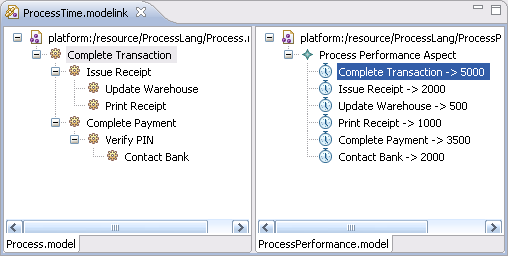
\includegraphics{images/ModeLink.png}
	\caption{Exemplar Process and ProcessPerformance models}
	\label{fig:ModeLink}
\end{figure*}

\begin{figure*}
	\centering
		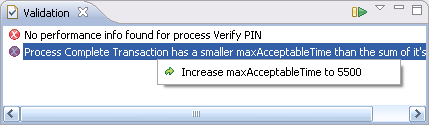
\includegraphics{images/Validation.png}
	\caption{Screenshot of the validation view reporting the identified inconsistencies}
	\label{fig:Validation}
\end{figure*}

To demonstrate the evaluation of these constraints two exemplar models that conform to the \emph{ProcessLang} and \emph{ProcessPerformanceLang} metamodels are used. A visual representation of the models is displayed in Figure \ref{fig:ModeLink}.

Evaluating the constraints in the context of those two models reveals two problems which are reported to the user via the view displayed in Figure \ref{fig:Validation}. Indeed by examining the two models of Figure \ref{fig:ModeLink}, it becomes apparent that there is no \emph{ProcessPerformance} linked to the \emph{Verify PIN} process and also that the \emph{maxAcceptableTime} of \emph{Complete Transaction} (5000) is less than the sum of the \emph{maxAcceptableTimes} of its children (2000 + 3500).

\section{Summary}

This section has provided a detailed discussion on the EVL model-validation language which conceptually (as opposed to technically) extends OCL. EVL provides a number of features such as support for detailed user feedback, constraint dependency management, semi-automatic transactional inconsistency resolution and (as it is based on EOL) access to multiple models of diverse metamodels and technologies.

%%% Local Variables:
%%% mode: latex
%%% TeX-master: "EpsilonBook"
%%% End:
